
%\section{Calibration and Validation}
\section{Validation}
\label{sec:validation}

%
% meshed vanes are 24x more expensive
%

The previous sections briefly outlined the physical regime under
consideration, the mathematical models we have developed to emulate
these conditions, and the software we are leveraging to solve these
equations for a variety of system configurations and scenarios. 
However, in order for our simulations to be useful for prediction, we
need to evaluate models against experimental data so
as to ensure that the entire formulation accurately reflects reality. 
Thus, this section discusses the validation of computational results
against existing experimental data and high fidelity simulations.

%
% experimental challenges
%
Several challenges arise in performing a validation study between the
simulation output and the experimental data. These data were taken using
particle image velocimetery (PIV), often not without non-trivial error
in measurement and sampling. 
The validation challenge is compounded by the fact that very little is
known about the uncertainties in the observation data. PIV is a
non-intrusive technique, but it does rely upon large sample sizes in
order to generate reliable statistics. While several hundred PIV
snapshots are available, no quantified uncertainties for the averaged fields
presently exist.  

In addition, only velocity measurements are available. Several
potentially important quantities of interest, such as the pressure field
or the temperature, have not been measured, and cannot then be used for
the purposes of validation. 


%
%\subsection{Model Calibration}
%
%
% viscosity calibrated
% 


\subsection{Model Validation}


  \begin{figure}[!htb]
    \begin{center}
     \includegraphics[width = 12 cm]{figs/lab_setup}
     \caption{The laboratory configuration, with straight vanes. The
     configuration is shown with a turbine, but it was removed for data
     gathering.}
     \label{fig:lab}
    \end{center}
  \end{figure}

\todo{mention georgia tech room}

These simulations are designed mimic the notional SoV experimental
facility to make direct comparisons between the output of simulation and
experimental measurement. The general system configuration is depicted
in Figure \ref{fig:lab}. 

The experimental laboratory has numerous objects
in the immediate vicinity (see figure \ref{lab}) that may
obstruct/manipulate the flow. These objects may be moved or removed
during PIV data gathering. The laboratory simulation uses adiabatic side
walls as a boundary condition. It is unclear how much of an impact this
may have on the simulation. It is also unclear if this is a realistic
boundary condition. 

While no sensitivity analysis has been performed, it is likely that the
largest uncertainty in the laboratory simulation is a result of the
ventilation. The heated plate on the bottom of the laboratory
generates enough heat to cause a significant increase in room
temperature (30+ Kelvin). This also greatly impacts the SoV
performance, as the ground to air thermal gradient drives the
vortex. The laboratory therefore utilizes cooling in order to maintain
temperature, in particular, two inlet HVAC ducts into the room. While
efforts have been made to characterize the level of ventillation being
used, these numbers come with non-trivial uncertainties attached. One
vent runs continuously at 288 Kelvin with a flow rate of approximately 1 
$m^3$/s.
%(4-6 m/s with an approximate area of 0.2 $m^2$)
The other vent initializes only if the room exceeds 301 Kelvin
Finally, the air is expected to leave through the laboratory doors.

We have attempted to mimic these scenario conditions in our
simulations. To do so, we impose Dirichlet boundary conditions to
establish a constant inflow condition of cool air at the rates 
proscribed by our collaborators. Prelimary results indicated that 
inflow rates consistent with the lower bound of those estimates result in an
unrealistic heating of the room, while inflow conditions at the high end
result in velocity profiles that exceed the laboratory measurements. In
other words, our simulations appear to be sensitive to the choice of
inflow rate, and it is likely that the laboratory is run where one of
the vents is operating intermittently. 

  \begin{figure}[!htb]
    \begin{center}
     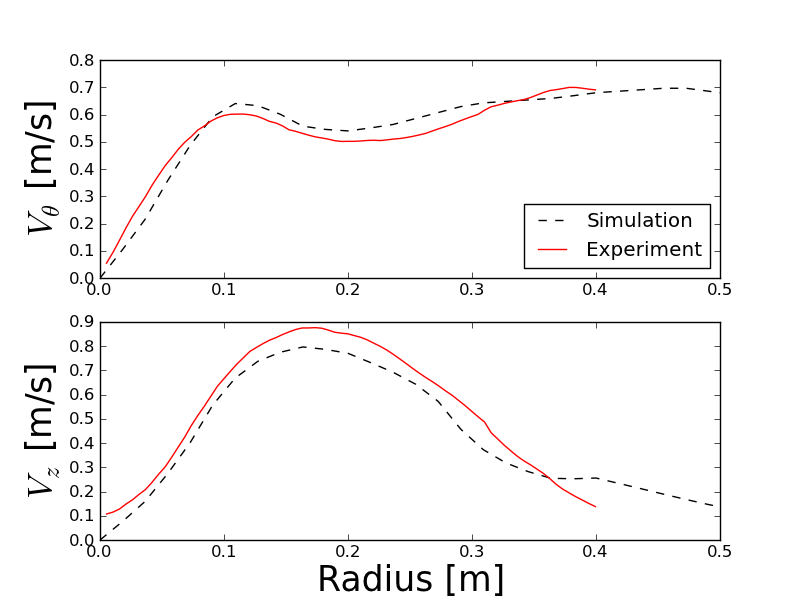
\includegraphics[width = 12 cm]{figs/hybrid_profile}
     \caption{add something about validation here}
     \label{fig:lab}
    \end{center}
  \end{figure}

%
%
%

Our initial focus has therefore moved to a validation study to ensure that the
output of the numerical simulation agrees with the experimental
measurements. The flows are qualitatively similar, with a vortex forming
in the center of in both cases, but the degree to which each matches
each other is unclear and must be characterized. 

In particular, we have implemented a simulation designed
to closely mimic the 30 degree vane experimental setup. The outputs of
the simulation (velocity field, temperatures, etc. ) are then compared
to available experimental data, which at this time is principally the
velocity field taken by PIV measurements at a variety of time frames
near the center of the SoV. This ``high-cost'' simulation resolves
the SoV large-scale structure, as well as the turning vanes
nearby. Comparisons must be made between the:
\begin{itemize}
 \item Azimuthal Velocity as a function of radius from center of the Sov
 \item Azimuthal Velocity as a function of the height at different
       points in the SoV
 \item Vertical Velocity as a function of radius from center of the Sov
 \item Vertical Velocity as a function of the height at different
       points in the SoV
\end{itemize}

%
% hybrid (embedded model)
%
Further validation cases are required. We are now in a position to perform
a validation of the embedded vane model. As described previously, this
uses the same turbulence models, but now without resolving the turning
vanes. Instead of resolving the vanes, for a region in the flow, the
velocity field is forced in a manner similar to as if the fluid was
moving through the turning vanes. While direct comparisons between this
model and the experimental data can be (and will be) made, a comparison
between this ``low-cost'' (in terms of computation and mesh
requirements) simulation and is useful for several reasons. It permits
directly comparing the effect of the simple, low cost, turning vane
model against the higher resolution modeling (essentially this permits a
validation of an embedded model). Furthermore, it allows us to observe a
much richer set of possible changes in the state space than in the
experiment, which is constrained to only velocity measurements. 


%\subsection{Further Concerns}
%
% no quantitative data from wind cases! 
%
% qualitative agreement between our results and wind tunnel
% agreement within ~15% of energy flux 
%


%
% turbine
%
Thus, this adds another significant validation case, with new, significant,
challenges in modeling the turbines. This is in essence a new embedded
submodel that we will add after validation of the initial configuration
is completed. 
